\documentclass[fleqn]{article}
\oddsidemargin 0.0in
\textwidth 6.0in
\thispagestyle{empty}
\usepackage{import}
\usepackage{amsmath}
\usepackage{graphicx}
\usepackage{flexisym}
\usepackage{amssymb}
\usepackage{bigints} 
\usepackage[english]{babel}
\usepackage[utf8x]{inputenc}
\usepackage{float}
\usepackage[colorinlistoftodos]{todonotes}

\definecolor{hwColor}{HTML}{AD53BA}

\begin{document}

  \begin{titlepage}

    \newcommand{\HRule}{\rule{\linewidth}{0.5mm}}

    \center


    \textsc{\LARGE Arizona State University}\\[1.5cm]

    \textsc{\LARGE Quantum Physics I }\\[1.5cm]


    \begin{figure}
      
\includegraphics[width=\linewidth]{asu.png}
    \end{figure}


    \HRule \\[0.4cm]
    { \huge \bfseries Homework Nine}\\[0.4cm] 
    \HRule \\[1.5cm]

    \textbf{Behnam Amiri}

    \bigbreak

    \textbf{Prof: Richard Kirian}

    \bigbreak


    \textbf{{\large \today}\\[2cm]}

    \vfill 

  \end{titlepage}
 
  \textbf{2.29} \\ \\
  Analyze the odd bound state wave functions for the finite square well. 
  Derive the transcendental equation for the allowed energies, and solve it
  graphically. Examine the two limiting cases. Is there always an odd bound state?

  \rule{15cm}{1pt}

  \textbf{2.31} \\ \\
  The Dirac delta function can be thought of as the limiting case of a
  rectangle of area 1, as the height goes to infinity and the width goes to zero. Show
  that the delta-function well (Equation 2.117) is a "weak" potential (even though it
  is infinitely deep), in the sense that $z \rightarrow 0$. Determine the bound state energy
  for the delta-function potential, by treating it as the limit of a finite square well.
  Check that your answer is consistent with Equation 2.132. Also show that
  Equation 2.172 reduces to Equation 2.144 in the appropriate limit.

  \rule{15cm}{1pt}
  
  \textbf{2.33} \\ \\
  Determine the transmission coefficient for a rectangular barrier
  (same as Equation 2.148, only with $V(x)=+V_0 >0$ in the region $-a<x<a$).
  Treat separately the three cases $E<V_0, ~ E=V_0, ~ $ and $E>V_0$ 
  (note that the wave function inside the barrier is different in the three cases).
  Partial answer: for $E<V_0$
  $$T^{-1}=1+\dfrac{V^2_0}{4E(V_0-E)} sinh^2 \left(\dfrac{2a}{\hbar} \sqrt{2m(V_0-E)}\right)$$


  \rule{15cm}{1pt}
  
  \textbf{2.40} \\ \\
  A particle of mass m in the harmonic oscillator potential (Equation
  2.44) starts out in the state
  $$\Psi(x,0)=A \left(1-2\sqrt{\dfrac{m \omega}{\hbar}}x\right)^2 ~ e^{-\dfrac{m\omega}{2\hbar} x^2}$$
  for some constant $A$.
  \begin{itemize}
    \item Determine $A$ and the coefficients $c_n$ in the expansion of this state in terms
    of the stationary states of the harmonic oscillator.

    \item In a measurement of the particle’s energy, what results could you get, and
    what are their probabilities? What is the expectation value of the energy?

    \item At a later time T the wave function is
    $$\Psi(x,T)=B\left(1+2\sqrt{\dfrac{m \omega}{\hbar}}x\right)^2 ~ e^{-\dfrac{m\omega}{2\hbar} x^2}$$
    for some constant B. What is the smallest possible value of $T$?
  \end{itemize}


  \rule{15cm}{1pt}
  
  \textbf{2.58} \\ \\
  In a monovalent metal, one electron per atom is free to roam
  throughout the object. What holds such a material together—why doesn’t it
  simply fall apart into a pile of individual atoms? Evidently the energy of the
  composite structure must be less than the energy of the isolated atoms. This
  problem offers a crude but illuminating explanation for the cohesiveness of
  metals.
  \begin{itemize}
    \item Estimate the energy of N isolated atoms, by treating each one as an
    electron in the ground state of an infinite square well of width a
    (Figure 2.23(a)).
    
    \item When these atoms come together to form a metal, we get N electrons in a
    much larger infinite square well of width Na (Figure 2.23(b)). Because of
    the Pauli exclusion principle (which we will discuss in Chapter 5) there
    can only be one electron (two, if you include spin, but let’s ignore that) in
    each allowed state. What is the lowest energy for this system
    (Figure 2.23(b))?

    \item The difference of these two energies is the \textbf{cohesive energy} of the metal—
    the energy it would take to tear it apart into isolated atoms. Find the
    cohesive energy per atom, in the limit of large N.


    \item Atypical atomic separation in a metal is a few Ångström (say, $a \approx 4 ~ \mbox{\normalfont\AA}$).
    What is the numerical value of the cohesive energy per atom, in this
    model? (Measured values are in the range of 2–4 eV.)

    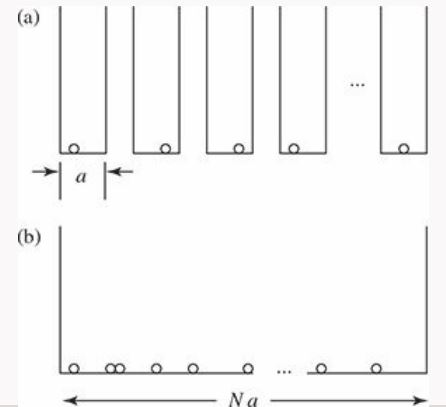
\includegraphics[height=6cm, width=10cm]{one.JPG}
    
  \end{itemize}


  \end{document}
